\documentclass{article}
\usepackage[english]{babel}
\usepackage[a4paper,top=2cm,bottom=2cm,left=2cm,right=2cm]{geometry}

\usepackage{amsmath}
\usepackage{graphicx}
\usepackage{subcaption}
\usepackage{booktabs}

\usepackage{natbib}
	\bibliographystyle{apalike}

\usepackage[colorlinks=true, allcolors=blue]{hyperref}
\usepackage{hyperref}
	\hypersetup{
		colorlinks=true,
		linkcolor=blue,
		filecolor=blue,
		urlcolor=blue,
		citecolor=blue
	}
\usepackage{acronym}

\title{Dock Door Case Study\\
\normalsize{in collaboration with Mojix}}
\author{Marlize DE VILLIERS \\
Ayoub YOUSSOUFI}

\pagenumbering{roman}

\begin{document}

\maketitle

\hrule

\tableofcontents

\listoftables\addcontentsline{toc}{section}{List of Tables}
\listoffigures\addcontentsline{toc}{section}{List of Figures}

\section*{Acronyms}
\addcontentsline{toc}{section}{Acronyms}
\begin{acronym}[ABCDEF]
\acro{RFID}{Radio-Frequency Identification}
\acro{IoT}{Internet of Things}
\acro{RSSI}{Received Signal Strength Indication}
\acro{RC}{Read count of the RSSI}
\acro{MLP}{Multi-layer perceptron}
\acro{EPC}{Electronic Product Code}
\acro{kNN}{k-Nearest Neighbours}
\acro{SVM}{Support Vector Machine}
\acro{SMOTE}{Synthetic Minority Oversampling TEchnique}
\end{acronym}

\clearpage

\pagenumbering{arabic}
\section{Introduction}

Industry 4.0 and the technology that comes with it has gained popularity over the last few years.
One innovative application of Industry 4.0 is inventory management, and specifically, the automation thereof.
In short, inventory management is concerned with monitoring stock as it arrives, moves around, and leaves the facility.
One way in which Industry 4.0 is playing a role in inventory management is by automating inventory management using \ac{RFID} technology.

Automated inventory management has recently became a point of interest for many businesses, since automated inventory management can save time, make people's jobs easier, and reduce the number of human errors made.
This all has a positive impact on the business's overall productivity and efficiency.
These aspects are all important for businesses who wish to remain competitive\,---\,especially in the time of Industry 4.0.

\subsection{Company background}

Mojix is a leading software company that focuses their building solutions for their customers\,---\,whether they are consumers, retailers, or industry enterprises\,---\,using data gathered by various \ac{IoT} technologies.
One of Mojix's focuses is digitizing and automating supply chains.
They do this in various ways.
This case study focuses on automated inventory management.
The way that Mojix has decided to approach this problem is using \ac{RFID} technology.

\ac{RFID} technology enables Mojix to automate an inventory system by allowing communication between \ac{RFID} tags and sensors.
Data are transmitted between the tags and the sensors, automating the process of monitoring stock in a facility without the need for humans to interfere or assist \citep{ref:about_mojix}.
Mojix already has item chain management solutions\,---\,shown in Figure \ref{fig:item_management_sol}\,---\,that help their clients manage the life-cycle of the products in terms of cost, time and quality of the operations to deliver unique end-to-end costumer experience.
%
\begin{figure}[h]
    \centering
    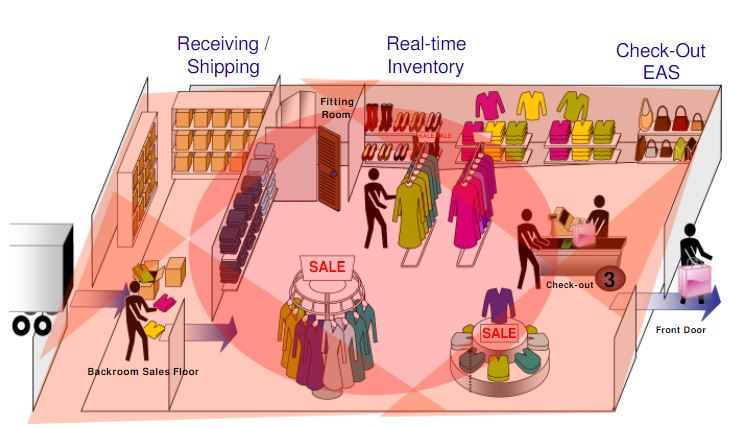
\includegraphics[scale = 0.6]{Images/mojix1.JPG}
    \caption{An example of an item management solution provided to clothing store \citep{ref:solutions_consultant}}
    \label{fig:item_management_sol}
\end{figure}
%

\subsection{Problem statement}

When this case study was started, the Dock Door project was very recently started at Mojix.
As a result, this case study contributed to refining the problem definition for Mojix since as work was done, new problems and ideas came up and were included into the scope.
The case study, therefore, aided in developing the project.
The final problem statement, therefore is:
\textit{Find a way to automate the inventory management system using machine learning without compromising on performance.}

From this problem statement, three main tasks were identified:
\begin{enumerate}
    \item Accurately distinguishing between moving and static \ac{RFID} tags.
    \item Accurately determine if moving tags are coming into the facility or leaving the facility.
    \item Accurately determine the time that tags entered or left the facility.
\end{enumerate}
This case study focuses mainly on these three tasks.

The rest of the report contains the \emph{Literature review} which discusses some technical concepts and previous work, followed by a description of the data used in the \emph{Dataset} section.
The algorithms used in the case study are briefly explained in the \emph{Algorithms} section.
Then, in the \emph{Results}, each problem identified in the problem statement is described and the machine learning algorithms' performances are discussed.
Lastly, the findings of this case study and our advice to Mojix regarding future work are contained in the \emph{Conclusion and recommendations}.

\section{Literature review}

The Industry 4.0 concept opens opportunities to digitize industrial machines, processes, and assets; providing new insights and efficiently counteracting various challenges. 
\ac{RFID} is a key Industry 4.0 enabling technology, and has been widely used throughout manufacturing and supply chain areas such as logistics, clothing industry, library management, warehouse management and so on, and object localization has always been a hot topic in \ac{RFID} research. 
In this section some concepts around \ac{RFID} will be discussed, along with the use of \ac{RFID} in inventory management, and finally, previous work on the same topic will be reviewed.

\subsection{Radio-frequency identification}

\ac{RFID} technology is systematically replacing barcode identification.
It simplifies and eliminates routine work of employees by manually detecting and identifying \ac{RFID} tags using antennas, by removing the need to manually locate and scan barcodes to identify products.
What makes \ac{RFID} especially useful, is that a direct line of sight to the tagged item is not required for the antennas to detect the tags.
Certain \ac{RFID} technology can work over distances greater 20m \citep{ref:about_rfid}.
All of this is why \ac{RFID} is particularly suited for inventory management.

An \ac{RFID} system comprises the following:
\begin{itemize}
    \item Tags
    \item Readers
    \item Antennas
\end{itemize}
The tags are attached to the products of interest, and consist of two parts, an antenna that can send or receive signals, and a chip which stores the information about the tag\,---\,or its identification.
Readers send and receive signals to and from the tags.
Antennas essentially convert the signals from the readers into radio-frequency waves so that tags can be detected\citep{ref:about_rfid}.

In short, the readers send signals, which are converted into radio-frequency waves by the antennas.
When the radio-frequency waves reach a tag, the wave is reflected back to the antenna on the same path.
The received radio-frequency wave is then converted back into a signal to enable the reader to receive the signal.
This process enables us to determine the distance of the tag using the \ac{RSSI}.
The \ac{RSSI} gives an indication of how strong the received signal is, which can then be used to determine the distance that the signal has travelled.

A main problem with the \ac{RSSI} (and of \ac{RFID} technology) is that the radio-frequency waves can ``echo'' and bounce off of metal surfaces. 
This becomes an even bigger problem in a closed environment, such as a warehouse.
Unfortunately, the \ac{RSSI} is the only measure available to determine the location of a tag relative to the readers, and if a more accurate location is required, it might be necessary to introduce additional technology \citep{ref:about_rssi}.
Similar to this, the readers have no way to determine if a tag is moving or static, since the \ac{RSSI} is a single value received at a time.

\subsection{Problems when using radio-frequency identification for inventory management}

In an inventory management system, an \ac{RFID} system can monitor tagged products moving through an entrance or exit of a warehouse. 
However, \ac{RFID} cannot distinguish signals received from tagged products that are actually moving through the gate from the signal that enter the reading range accidentally because of interference.
This gives rise to a common problem in an \ac{RFID} inventory management system\,---\,distinguishing true positives from false positives (i.e.: static tags are accidentally detected as moving tags are false positives, and are not of interest to the business process at the time that they are static.)
Tags that move through the entrance or exit are called true positives.

In an attempt to minimise this problem, Mojix has a dedicated ``in zone'' and a dedicated ``out zone'', along with an ``in antenna'' aimed at the ``in zone'', and an ``out antenna'' aimed at the ``out zone''.
The setup is shown in Figure \ref{fig:dock_door}.
%
\begin{figure}[h]
    \centering
    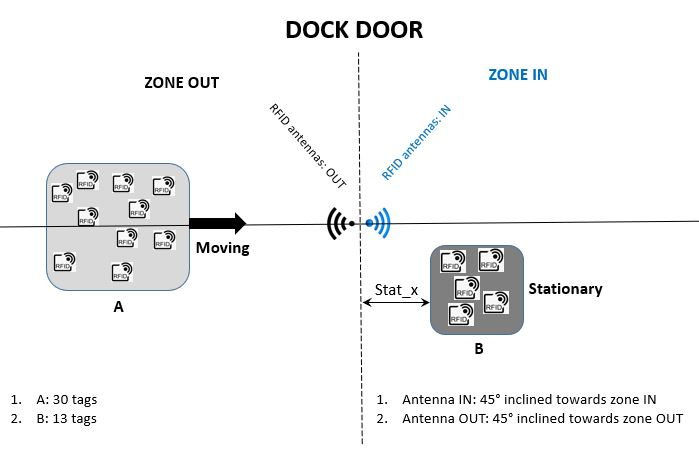
\includegraphics[scale = 0.65]{Images/mojix2.JPG}
    \caption{RFID system setup at the dock door in the warehouse \citep{ref:about_mojix}.}
    \label{fig:dock_door}
\end{figure}
%
Though this does decrease false positives a little bit, it does not eliminate them completely.
It also gives rise to an additional definition of false positives and false negatives: tags in a specific zone being detected by the other zone's antenna.
This happens because of the echoing and interference discussed in the previous subsection.

\subsection{Using machine learning to solve the problems posed by radio-frequency identification}
Using machine learning for inventory management with \ac{RFID} is not a new concept, but the literature is limited.
Nonetheless, some insightful work has been done.
The work that was done for this case study was mostly inspired by the first paper mentioned in this subsection.

\citet{ref:Alfian} used machine learning combined with \ac{RFID} to improve the traceability of items in a supply chain.
In their study, it was important to be able to determine the direction of movement of the \ac{RFID} tags\,---\,since they wanted to be able to accurately track and trace items in the warehouses in the supply chain.
The problem they tried to solve is very similar to the problem Mojix is trying to solve.

\citet{ref:Alfian} approached the problem by gathering data of various tag movements, namely:
\begin{enumerate}
    \item Move from inside to outside.
    \item Move from outside to inside.
    \item Move around inside or move around outside.
    \item Static inside or static outside.
\end{enumerate}
The data that they gathered was the \ac{RSSI} of the tags and the time the \ac{RSSI} was received.
They gathered the data for the tags being moved at various speeds, and the movement of tags going through the gate was always from 5m inside the one zone to 5m inside the other zone.
After the data were gathered, they labeled the data appropriately according to the tags movements.
The data thus contained, per run (a run is one completed movement of the tags), the following:
\begin{enumerate}
    \item The timestamp.
    \item The tag's identification.
    \item The \ac{RSSI}.
    \item The antenna that received the \ac{RSSI}.
    \item The movement class.
\end{enumerate}

Figure \ref{fig:Alfian_setup} shows the \ac{RSSI} of the tags during various movements.
%
\begin{figure}[h]
    \centering
    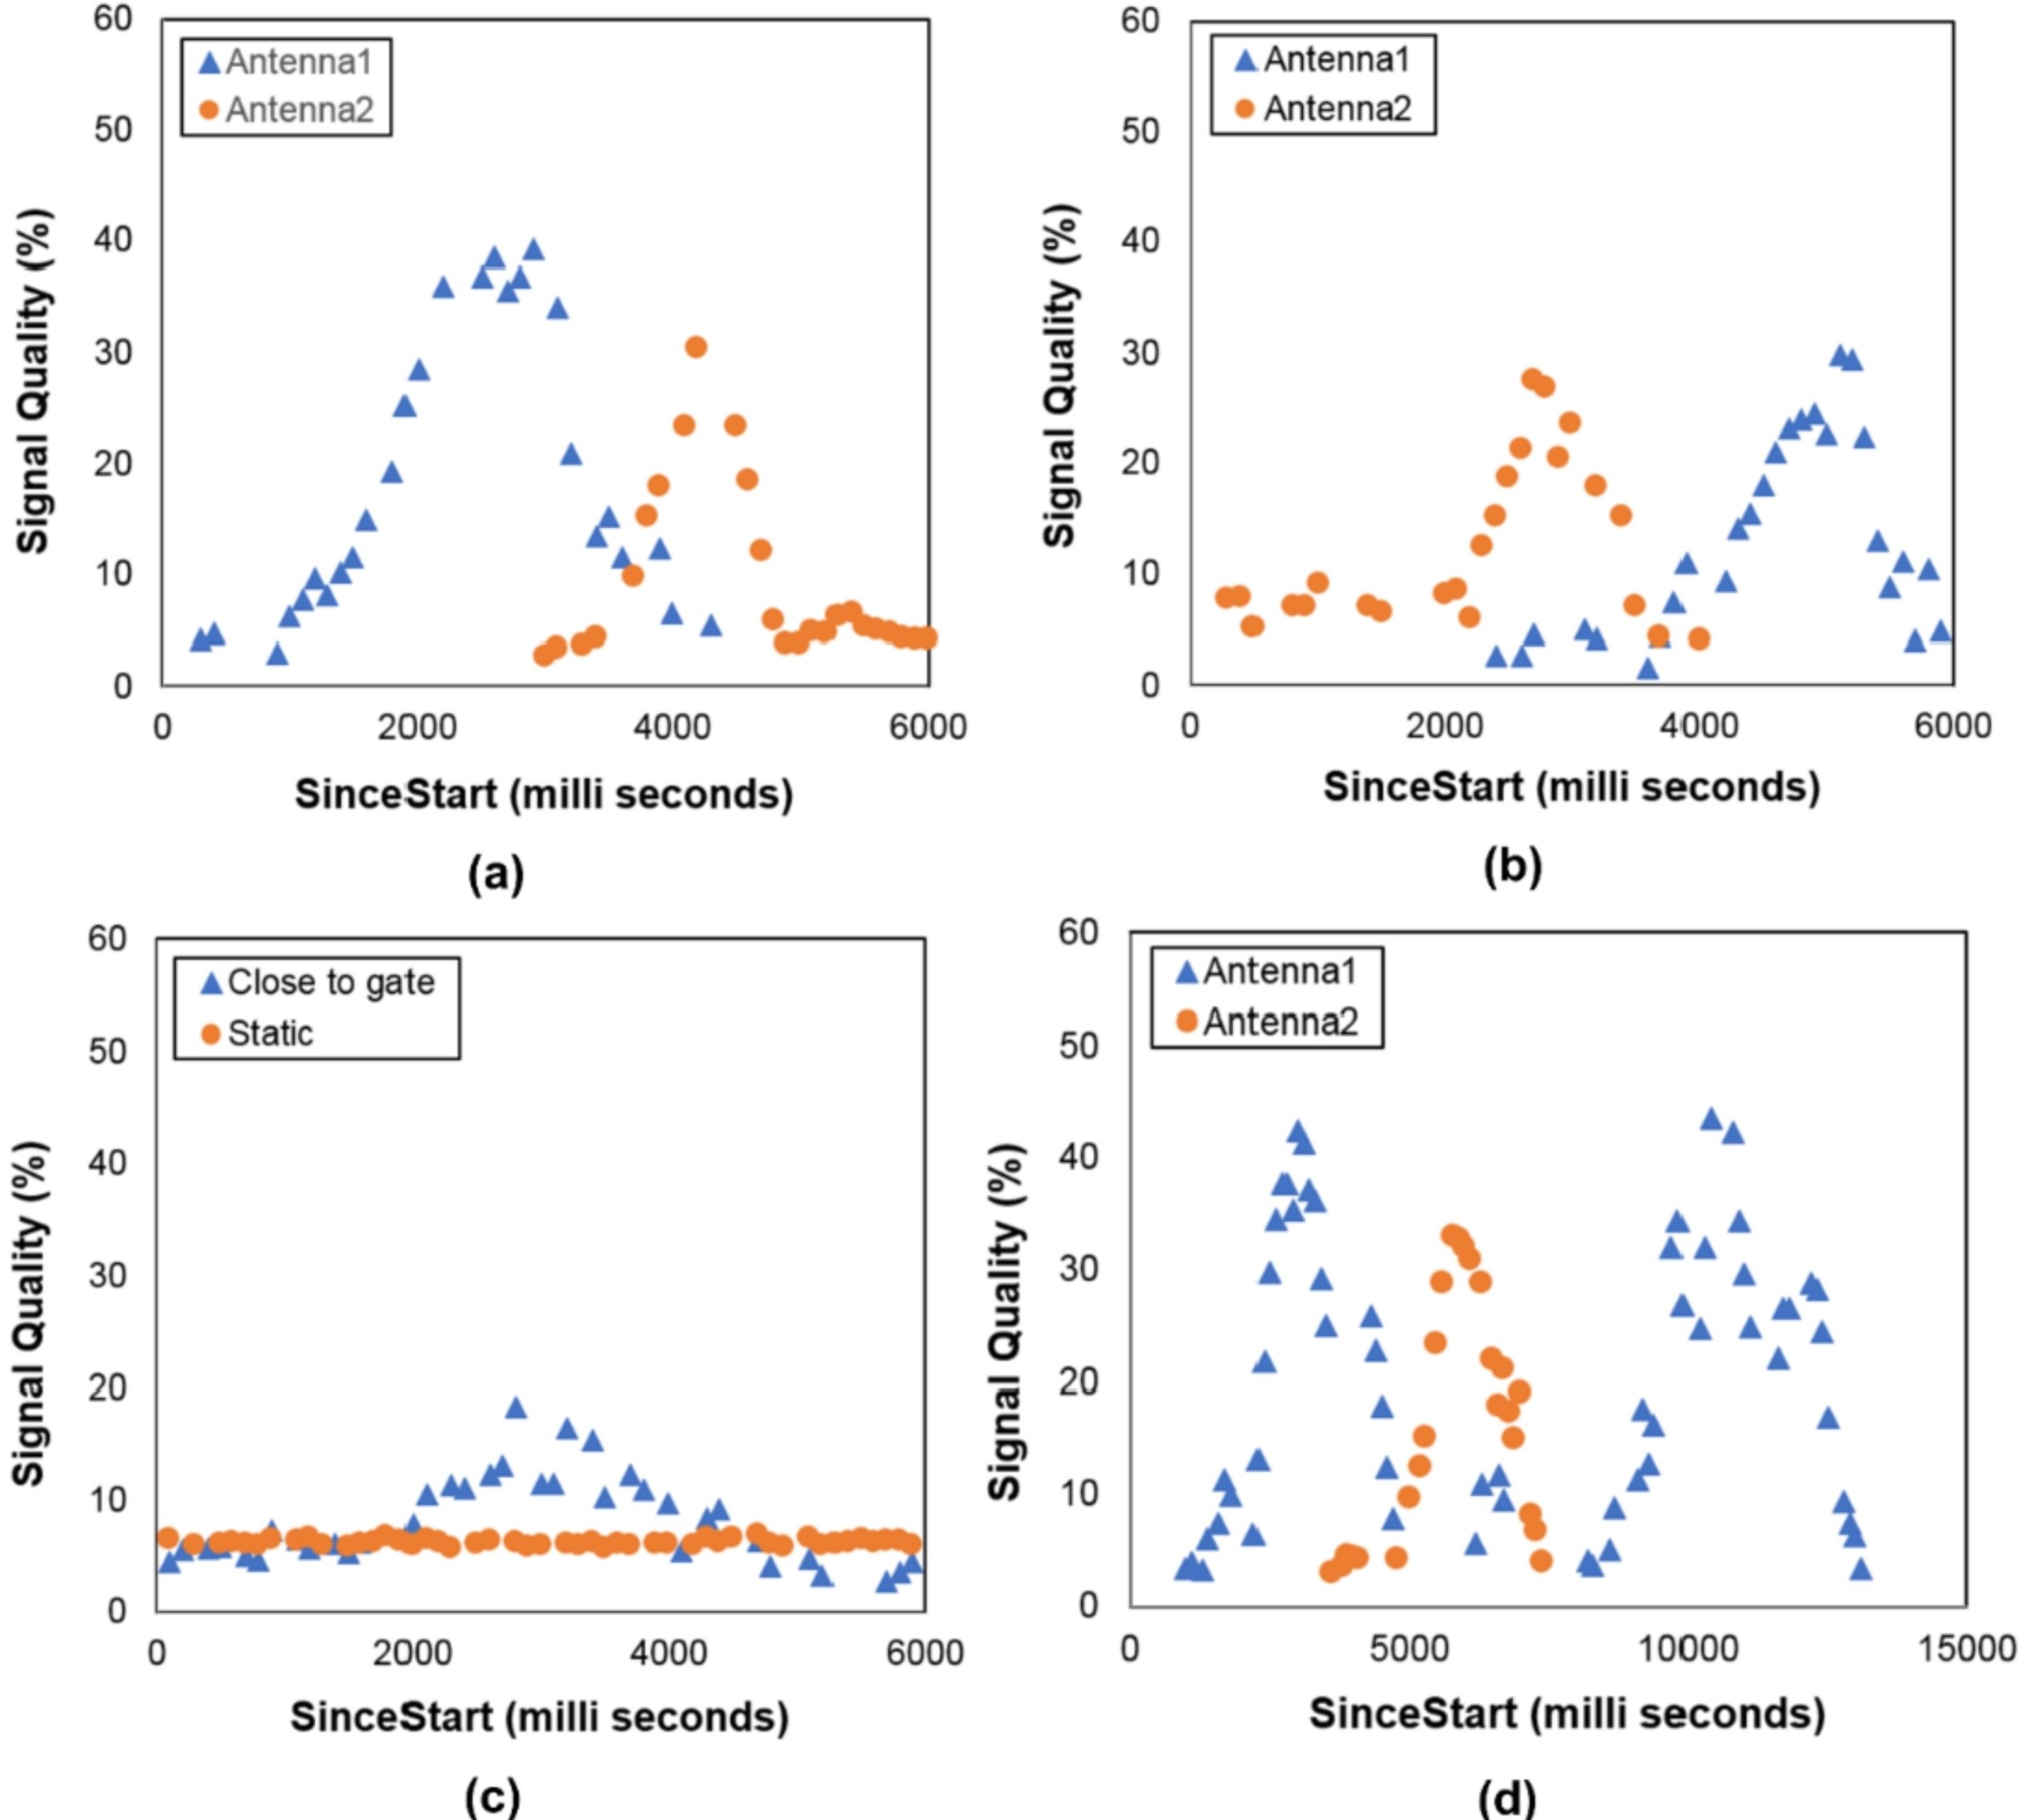
\includegraphics[scale = 1]{Images/tag movement graphs.jpg}
    \caption{RSSI of the tags in the experimental setup of \citet{ref:Alfian}.}
    \label{fig:Alfian_setup}
\end{figure}
%
Sub-figure a shows tags moving from outside to inside, and subfigure b shows tags moving from inside to outside.
Sub-figure c shows tags moving around outside, and static tags inside, and sub-figure d shows tags moving inside close to the gate and then away again\,---\,without actually crossing the gate.
We can see as the tags move through (or close to) the gate, the \ac{RSSI} increases and they are first detected by one antenna, and as they approach, the \ac{RSSI} for the first antenna decreases and they start to be detected by the second antenna with an increasing \ac{RSSI}.
If they move through, eventually, they are only detected by the second antenna.
Static tags have a constant \ac{RSSI}, and tags that move within one zone have a smaller maximim \ac{RSSI}.
If tags move close to the gate and then away again, they are detected twice by the first antenna with a strong \ac{RSSI}, and once by the second antenna with a slightly weaker \ac{RSSI}.

\citet{ref:Alfian} used numerous machine learning algorithms.
They found that some algorithms performed better than others, with the best performance being that of the XGBoost algorithm, and the poorest performance from the \ac{MLP}.
Their results are shown in Table \ref{tab:alfian_results}.
%
\begin{table}[h!]
\centering
\setlength{\belowcaptionskip}{7pt}
\caption{Results obtained by \citet{ref:Alfian}.}
\label{tab:alfian_results}
\begin{tabular}{@{}lrrrr@{}}
\toprule
\multicolumn{1}{c}{\textbf{Algorithm}} & \multicolumn{1}{c}{\textbf{Accuracy}} & \multicolumn{1}{c}{\textbf{Precision}} & \multicolumn{1}{c}{\textbf{Recall}} & \multicolumn{1}{c}{\textbf{F1-score}} \\ \midrule
\ac{MLP}                                & 63.59\%                           & 62.03\%                                         & 59.13\%                           & 55.73\%                               \\
Logistic regression                    & 80.10\%                               & 80.08\%                                & 78.01\%                             & 77.45\%                               \\
K-nearest neighbors                    & 66.70\%                               & 64.35\%                                & 62.35\%                             & 62.32\%                               \\
Decision tree                          & 66.99\%                               & 61.89\%                                & 63.57\%                             & 58.58\%                               \\
Naive Bayes                            & 73.30\%                               & 75.22\%                                & 70.38\%                             & 70.51\%                               \\
Random forest                          & 92.72\%                               & 92.64\%                                & 92.04\%                             & 91.96\%                               \\
AdaBoost                               & 92.43\%                               & 92.13\%                                & 91.80\%                             & 91.64\%                               \\
XGBoost                                & 93.59\%                               & 93.25\%                                & 92.95\%                             & 92.78\%                               \\ \bottomrule
\end{tabular}
\end{table}
%
The performance of the XGBoost algorithm looks promising, but Mojix would like to see if they can get an even better performance.

In the problem statement it was mentioned that detecting false positives is also important since false positives have a negative impact on the accuracy of an \ac{RFID} inventory management system.
\citet{ref:Ma} investigated algorithms to identify false positives in an \ac{RFID} readings.
The data they used to do this, was more descriptive than the data used by \citet{ref:Alfian}. 
For example, they used summary statistics of individual tags' \ac{RSSI}, such as, the maximum and minimum \ac{RSSI}, the mean \ac{RSSI}, the \ac{RSSI}'s range, variance and skewness, to give an idea.
The purpose of this is because tags doing different movements, will give different \ac{RSSI} patterns.
For example, static tags will have a constant \ac{RSSI}, meaning the maximum, minimum, and mean \ac{RSSI} will be very close, and there will be very little variance in the \ac{RSSI}.
A tag that moves around in a zone will have a varying \ac{RSSI}, but the maximum \ac{RSSI} will be lower than the maximum \ac{RSSI} of a tag that moves through the gate.

\citet{ref:Ma} compared three algorithms to detect false positives.
The results are as follows:
\begin{itemize}
    \item 92.75\% accuracy for false positive detection using logistic regression.
    \item 95.30\% accuracy for false positive detection using support vecor machine.
    \item 92.85\% accuracy for false positive detection using decision tree.
\end{itemize}
These results are promising, since no extra hardware was used to detect false positives.
However, during the case study, Mojix came up with an idea that decreased false positives significantly.
They proposed that the static tags be place at fixed distances from the dock door.
They gathered data from runs with static tags at distances of 1m, 3m, and 5m away from the dock door.
Using the distances of 3m and 5m effectively reduced the number of false positives without needing to use additional hardware.
This is because by placing the tags further from the antennas, the \ac{RSSI} of the static tags is significantly lower, and therefore, machine learning algorithms less frequently classify the static tags as moving tags.

\section{Datasets}

This section provides information on how the datasets used for the machine learning, look, but it does not go into fine details.
It some of the final datasets were constructed in very complex ways, taking inputs from multiple other datasets.

\subsection{Description}

In order to analyze the movement of the tags through the dock door, a dataset containing a large amount of information has been put together.
The data read by the antennas are structured in a table with 291\,510 rows and 28 columns, with the most important ones for this case study being: `\ac{EPC}', `run',`Timestamp', `Antenna', `\ac{RSSI}'.
Figure \ref{fig:init_data} shows the first few rows of the initial dataset.
%
\begin{figure}[h]
    \centering
    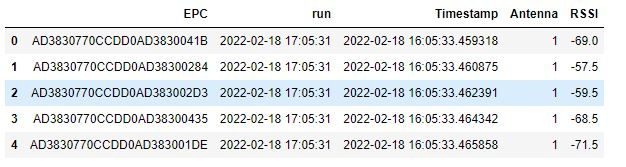
\includegraphics[scale = 0.7]{Images/mojix3.JPG}
    \caption{The first five rows of the dataset.}
    \label{fig:init_data}
\end{figure}
%
Each \ac{RFID} tag has a unique `\ac{EPC}', and this is the data that the antennas gather when a signal is received.
The `run' corresponds to when the recording of tag movements started.
The time that a tag is detected by an antenna is recorded in the `timestamp'.
Then, the data is integrated from the servers attached to the antennas in a database. 
This data is recorded in milliseconds shown in the `Timestamp' column.
`Antenna' corresponds to which antenna received the signal\,---\,1 is the antenna located in the `inside' zone and 2 is the antenna located in the `outside' zone. 
`\ac{RSSI}' is the strength of the signal received by the antenna.
Each antenna can, and does, read a unique \ac{EPC}s multiple times.
When the tag moves through the dock door, the other antenna will start to read the \ac{EPC} more frequently.

Next, there is a dataset containing information on each run.
Since each run was concerned with one type of tag movement, and there are 72 runs, this dataset contains 72 rows. 
The most important columns of this dataset are the direction of the moving tags, from which zone to which zone the tags are moving, the distance inside the zones the motion starts and stops, in which zone the static tags are and also how far inside each zone the static tags are located.
These columns are shown in Figure \ref{fig:runs_data}.
%
\begin{figure}[h]
    \centering
    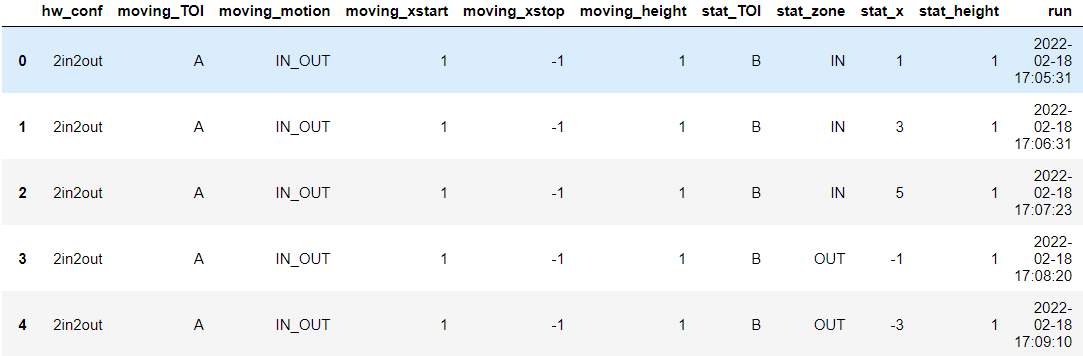
\includegraphics[scale = 0.5]{Images/runs.PNG}
    \caption{The first five rows of the runs dataset.}
    \label{fig:runs_data}
\end{figure}
%

Another necessary task was to determine when the tags moved out of one zone and into the other.
Mojix came up with the idea to use a sensor that emits a constant signal at the dock door.
The signal gets interrupted when the box or pallet with the tags crosses the line of signal, and the signal is received again when the box is done crossing the line of the signal.
The sensor records the time of the signal interruption and resumption, and this then becomes the time that the tags moved from one zone to the other.
These times were recorded in the gpio dataset, which is shown in Figure \ref{fig:gpio_data}.
%
\begin{figure}[h]
    \centering
    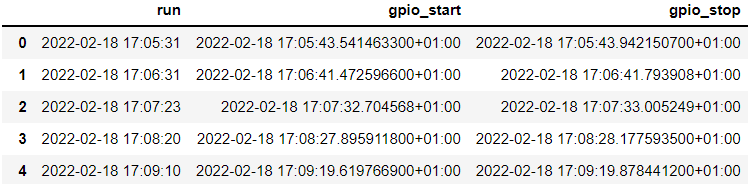
\includegraphics[scale = 0.7]{Images/gpio.PNG}
    \caption{The first five rows of the gpio dataset.}
    \label{fig:gpio_data}
\end{figure}
%
The `gpio\_start' column indicates the timestamps the tags started crossing the dock door, and the `gpio\_stop' column indicates the timestamps the tags finished crossing the dock door.

All of these datasets were merged to create one dataset that contains all of the required information, \emph{per tag}.
Since there are multiple tags in one box or on one pallet, the movement for many tags are the same per run.
The next subsection details some of the data preprocessing that was done.

\subsection{Cleaning and pre-processing}
Cleaning and pre-processing the data is a process done before analyzing it. Indeed, within this step, new features are created to be used in the deep learning and machine learning algorithms detailed in the next section.
\ac{RSSI} depends on the distance between the antenna and the \ac{EPC} tag.
Higher \ac{RSSI} signal indicate that the \ac{EPC} tag is moving very close to the antenna. 
Therefore, the \ac{RSSI} is a key element to identify the moving tags and the static ones. 
Table \ref{tab:RSSI_attributes} shows a summary of the \ac{RSSI} measurement data that were integrated into the previous data.
%
\begin{table}[h!]
\centering
\setlength{\belowcaptionskip}{7pt}
\caption{Different \ac{RSSI} attributes  }
\label{tab:RSSI_attributes}
\begin{tabular}{@{}ll@{}}
\toprule
\multicolumn{1}{c}{\textbf{Attribute Name}} & \multicolumn{1}{c}{\textbf{Description}} \\ \midrule
\ac{RSSI} MIN       & The minimum of all \ac{RSSI} values of a tag. \\
\ac{RSSI} MAX       & The maximum of all \ac{RSSI} values of a tag.  \\
\ac{RSSI} AVE       & The average of all \ac{RSSI} values of a tag.   \\
\ac{RSSI} LINMAX    & The maximum of all linear \ac{RSSI} values of a tag. \\
\ac{RSSI} LINAVE    & The average of all linear \ac{RSSI} values of a tag.  \\
\ac{RSSI} LINMIN    & The minimum of all linear \ac{RSSI} values of a tag. \\
\ac{RC}          & The number of time an \ac{EPC} is detected.     \\
\bottomrule
\end{tabular}
\end{table}
%

All of these 7 new features are concatenated and grouped by antenna coverage, to create in total 49 features that will be used by the machine learning models detailed in the next section \emph{Algorithms}.
%
\begin{figure}[h]
    \centering
    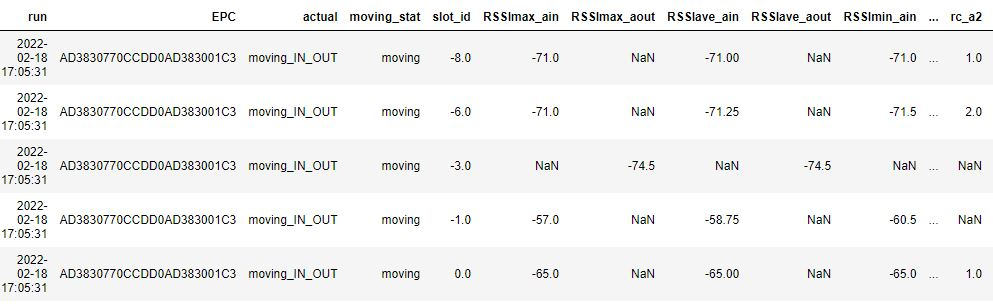
\includegraphics[scale = 0.5]{Images/ds_ml.JPG}
    \caption{The first five rows of the dataset used in  \emph{Algorithms} section.}
    \label{fig:final_dataset_without_windows}
\end{figure}
%

Next, a rolling window is joined to the table above. 
It shows one-second time slots per run. 
Each \ac{EPC} might be detected in multiple time slots. 
For machine learning, we are more interested in keeping only the winning windows where the \ac{EPC} is actually moving in/out through the dock door.
Mojix has gathered the data in such a way that the crossing will always occur in the [-2,-1,0,1] time slot.
Time slot 0 is where the crossing occurred, -2 is two seconds before the crossing, 1 is one second after the crossing etc.
This means that the final data-frame contains the 49 features of each \ac{EPC} during the [-2,-1,0,1] time slot, whether the \ac{EPC} is moving or static. 
In addition, a binary classification of \emph{moving} or \emph{static} is applied to each \ac{EPC}. 
This classification is the target feature of the predictive models explained in the \emph{Algorithms} section.
%
\begin{figure}[h]
    \centering
    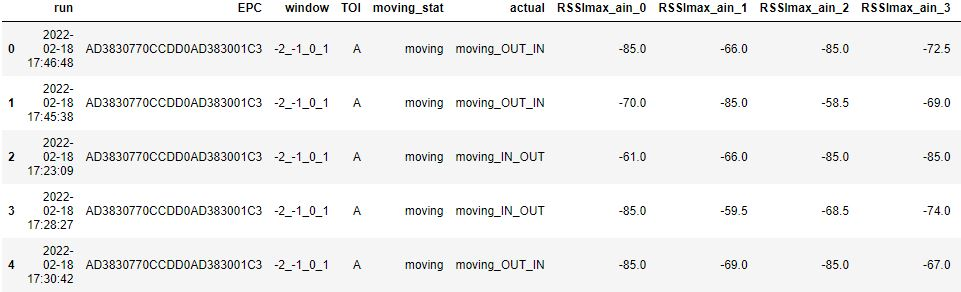
\includegraphics[scale = 0.5]{Images/final_data.JPG}
    \caption{The first 5 rows of the dataset with the wining crossing-windows used in \emph{Algorithms} section.}
    \label{fig:final_dataset}
\end{figure}
%

\section{Algorithms}

All of the algorithms used in this case study are briefly explained in this section.
Finer details about hyper-parameters are given in the \emph{Results} section.

\subsection{k-Nearest Neighbors}

\ac{kNN} is a supervised machine learning algorithm that can be used for both regression and classification. 
With a given new observation, \ac{kNN} can classify the new unlabelled observation by analysing k observations closest to the new observation.
In classification, the new observation is assigned the class that most of the k-nearest neighbors belong to, and in regression the new observation is assigned the mean of the k-nearest neighbors.
Therefore, k is a hyper-parameter that is fixed during the training of the algorithm \citep{christopher_2021}.

\subsection{Support Vector Machine}

\ac{SVM} is a supervised learning algorithm which can also be used for classification and regression.
It uses the kernel trick to transform the data into a higher dimension and then based on these transformations it finds an optimal decision boundary that maximises the distance between the different classes (in the case of classification.
New observations are assigned the same class of the observations on the same side of the decision boundary \citep{yadav_2018}.

\subsection{XGBoost}

XGBoost has recently became one of the most popular machine learning algorithms. 
It often provides good accuracies when other machine learning algorithms perform badly. 
It is often the go-to algorithm in modern-day machine learning problems. 
In some cases, XGBoost can be more efficient than the random forest, which was the state-of-the-art machine learning algorithm for very long. 
It is from the family of boosting algorithms. 
It works by training a fixed number of weak classifiers\,---\,often decision trees with one or two levels\,---\,and after one classifier is trained on the data, the next one is trained but preference is given to correctly classify the points that were wrongly classified by the previous classifiers \citep{seif_2022}.

\subsection{Neural Network}
Neural networks get their names because they emulate how the human brain works.
Many neurons are interconnected and transmit information to each other. 
Neural networks in machine learning is a network of neurons.
It starts with an input layer, and ends with an output layer, and has at least one hidden layer in between. 
All of these layers contain one or more neurons.
Each hidden layer processes the data coming from the previous layer to predict a specific target value, with the input layer taking the raw data, and the output layer outputting the prediction.
Neural networks may perform well when dealing with sophisticated data which generally does not perform too well with tranditional machine learning algorithms \citep{neuronetwork_2019}.

\section{Results}

In the final dataset that was set up for the machine learning, there are 2\,136 rows and 251 columns.
The normal \texttt{train\_test\_split} function was used to split the data.
The testing data were 33\% of the entire dataset and the training data were the remaining 67\%.
The final data also only includes the linear \ac{RSSI} values since Mojix determined through an analysis that the linear data produce better results than the non-linear data.

\subsection{Moving versus static tags}

In this specific task, the column `moving\_stat' was the target feature since it contains information on if a tag is moving or static.
The dataset is unbalanced on this feature, with 1\,760 moving observations and 376 static observations.

To determine if the tags are moving or static, classification machine learning algorithms were used.
Specifically, the \ac{kNN}, \ac{SVM}, XGBoost algorithms, and a neural network were used and their performance compared.
For the \ac{kNN} algorithm, k was set equal to 3 and 5, and the performance was compared.
For the \ac{SVM}, the C-parameter was set to 10, the gamma-parameter was set to 0.01, and a radial basis kernel was chosen.
These values were established through a grid search.
For XGBoost, the number of weak classifiers (single-level decision trees) was set to 100, and the learning rate was set to 1.
For the neural network, the feature-values were scaled using the \texttt{MinMaxScaler} and the labels were one-hot-encoded.
The network has an input layer, then 3 hidden layers with 32 neurons in each layer. 
A dropout rate of 0.25 was used to prevent overfitting.
The Adam optimiser was used with a learning rate of 0.0001.

The performance of the algorithms are shown in Table \ref{tab:Mov_stat_clas}.
%
\begin{table}[h!]
\centering
\setlength{\belowcaptionskip}{7pt}
\caption{Performances to predict if tags are moving or static.}
\label{tab:Mov_stat_clas}
\begin{tabular}{@{}lrrrrcc@{}}
\toprule
\multicolumn{1}{c}{\textbf{Algorithm}} & \multicolumn{1}{c}{\textbf{Accuracy}} & \multicolumn{1}{c}{\textbf{Precision}} & \multicolumn{1}{c}{\textbf{Recall}} & \multicolumn{1}{c}{\textbf{F1-score}} & \multicolumn{1}{c}{\textbf{False positives}} & \multicolumn{1}{c}{\textbf{False negatives}}\\ \midrule
kNN (k = 3)    & 94.18\%   & 94.40\%   & 94.18\%   & 94.27\%   & 25   & 16  \\
kNN (k = 5)    & 94.61\%   & 94.84\%   & 94.61\%   & 94.69\%   & 24   & 14  \\
SVM            & 97.45\%   & 97.49\%   & 97.45\%   & 97.46\%   & 11   & 7 \\
XGBoost        & 97.87\%   & 97.86\%   & 97.87\%   & 97.85\%   & 4    & 11  \\
Neural network & 97.45\%   & 97.47\%   & 97.45\%   & 97.46\%   & 10   & 8 \\ \bottomrule
\end{tabular}
\end{table}
%
The \ac{kNN} algorithm with k = 5 performs better than for k = 3.
The \ac{SVM} outperforms the \ac{kNN} algorithms in all of the metrics.
The neural network's performance is the same as the \ac{SVM} and also better than the \ac{kNN}.
The best performance was obtained by the XGBoost algorithm.
Particular attention should be paid to the number of false positives and false negatives. 
False positives are static tags that were predicted to be moving and false negatives are moving tags that were predicted to be static.
Both errors are equally bad in an inventory management setup, since it the higher the number of these errors are, the less accurate the inventory management system will be.
Therefore, the best algorithm for this task, is the XGBoost algorithm.
The confusion matrices for the algorithms and the neural network's training and validation loss graphs are shown in Figure \ref{fig:cm_mov_stat} in Appendix \ref{appendix:CM1}.
The it can be seen that the performance of the algorithms are similar, and that the XGBoost algorithm outperforms all of the other algorithms.

It should be noted that though these results are good, it is still a bit lower than the ideal.
In the next sub section, this classification problem is refined a bit by being more specific with the classes.

\subsection{Direction of moving tags and location of static tags}

In this specific task, the column `actual' was the target feature since it contains information on the tags' movement and locations.
The dataset is unbalanced on this feature, with 880 moving in to out observations, 880 moving out to in observations, 209 static in observations, and 167 static out observations.
For this task, the same algorithms were used, but the classification problem is now a multi-label classification problem.
The possible labels are:
\begin{itemize}
    \item moving\_in\_out
    \item moving\_out\_in
    \item static\_in
    \item static\_out
\end{itemize}
The only algorithm that changed was the neural network.
For this task it has an input layer, 3 hidden layers with 64 neurons each, and a dropout rate of 0.4 to prevent overfitting.

The results for this task is shown in Table \ref{tab:Mov_dir_stat_loc_clas}.
%
\begin{table}[h!]
\centering
\setlength{\belowcaptionskip}{7pt}
\caption{Performances to predict the direction of moving tags and the location of static tags.}
\label{tab:Mov_dir_stat_loc_clas}
\begin{tabular}{@{}lrrrr@{}}
\toprule
\multicolumn{1}{c}{\textbf{Algorithm}} & \multicolumn{1}{c}{\textbf{Accuracy}} & \multicolumn{1}{c}{\textbf{Precision}} & \multicolumn{1}{c}{\textbf{Recall}} & \multicolumn{1}{c}{\textbf{F1-score}} \\ \midrule
kNN (k = 3)    & 86.38\%   & 86.49\%   & 86.38\%   & 86.41\%  \\
kNN (k = 5)    & 87.66\%   & 87.89\%   & 87.66\%   & 87.72\%  \\
SVM            & 92.06\%   & 92.53\%   & 92.06\%   & 92.14\%  \\
XGBoost        & 91.63\%   & 91.76\%   & 91.63\%   & 91.64\%  \\
Neural network & 92.06\%   & 92.48\%   & 92.06\%   & 92.12\%  \\ \bottomrule
\end{tabular}
\end{table}
%
Similar as the previous task, the \ac{kNN} algorithms perform the worst.
The XGBoost algorithm performs better than the \ac{kNN}.
For this task, the \ac{SVM} and neural network give the best performances and their performances are very similar.
The results are again not as good as desired, but various hyperparameters were tried, and these are the best results.
The confusion matrices for the algorithms and the neural network's training and validation loss graphs are shown in Figure \ref{fig:cm_in_out} in Appendix \ref{appendix:CM2}.
The it can be seen that the performance of the algorithms are similar, and that the \ac{SVM} and neural network algorithms perform similar and outperform the other algorithms.

\subsection{Time tags move through the dock door}

The dataset used for this task contains 644 rows along with an analytically-determined (by Mojix) label called `actual', with possible values: `crossing' and `no crossing'.
The aim is for Mojix to further develop this task to include timestamps of each \ac{RSSI} reading, and using those timestamps to predict when the tags crossed the dock door, and along with task 2, to determine if the tags moved from inside the warehouse to outside, or \emph{vice versa}.
The dataset is severely unbalanced with 32 `crossing' labels and 612 `no crossing' labels.
After some preliminary experimentation, it was found that all of the algorithms simply predicted `no crossing' for all of the data because of how imbalanced the feature is.
To combat this problem, \ac{SMOTE} was used to oversample the `crossing' class in only the \emph{training} dataset, after using \texttt{train\_test\_split} with a test size of 40\%.
After using \ac{SMOTE}, the training data were balanced, containing 367 observations of both labels.

The performance was still not fantastic, because the testing data was still unbalanced, but there was a slight improvement.
The results are shown in Table \ref{tab:crossing_clas}.
%
\begin{table}[h!]
\centering
\setlength{\belowcaptionskip}{7pt}
\caption{Performances to predict if tags crossed the dock door.}
\label{tab:crossing_clas}
\begin{tabular}{@{}lrrrrcc@{}}
\toprule
\multicolumn{1}{c}{\textbf{Algorithm}} & \multicolumn{1}{c}{\textbf{Accuracy}} & \multicolumn{1}{c}{\textbf{Precision}} & \multicolumn{1}{c}{\textbf{Recall}} & \multicolumn{1}{c}{\textbf{F1-score}} & \multicolumn{1}{c}{\textbf{False positives}} & \multicolumn{1}{c}{\textbf{False negatives}}\\ \midrule
kNN (k = 3)    & 90\%   & 60\%   & 69\%   & 63\%  &  19  &  7  \\
kNN (k = 5)    & 89\%   & 60\%   & 72\%   & 63\%  &  23  &  6  \\
SVM            & 95\%   & 47\%   & 50\%   & 49\%  &  0  &  13  \\
XGBoost        & 96\%   & 86\%   & 61\%   & 67\%  &  1  &  10  \\
Neural network & 79\%   & 53\%   & 60\%   & 52\%  &  46  &  8  \\ \bottomrule
\end{tabular}
\end{table}
%
Even though the performance metrics are all close to or above 90\%, it should be noted that there were only 13 positive (crossing) labels in the testing data, so by looking at the false positives and false negatives numbers, it is evident that the performance is not good.
The confusion matrices of the algorithms and the loss graph of the neural network are shown in Figure \ref{fig:cm_crossing} in Appendix \ref{appendix:CM3}.
It is evident that the \ac{SVM} is not at all able to determine when tags cross the dock door, and the XGBoost and neural network cannot always determine when a crossing occurred.
The \ac{kNN} algorithms have more true positives, but at the expense of much more false positives.
This task's definition likely still needs to be defined better to be able to obtain better results.

\section{Conclusion and recommendations}

In this last section we briefly discuss the conclusions that were made during the case study.
We also give some recommendations that Mojix can consider for future work on this case study if they want to.

\subsection{Conclusion}

The first two tasks, determining if tags are moving or static and determining the direction of movement or location for static tags, are well defined, and similar porblems have been investigated in literature.
Specifically for the first task, determining if tags are moving or static, the results obtained are similar to those obtained in the study done by \citet{ref:Alfian}, which is that XGBoost has the best performance, but the \ac{SVM}'s and neural network's performances are very comparable to XGBoost's performance in this case study.

The second task, determining the direction of movement or location for static tags, is similar to the problem in the study by \citet{ref:Alfian}, but the results obtained in this case study is different.
In this case study the neural network and \ac{SVM} had superior performances, whereas \citet{ref:Alfian} found that their neural network had the worst performance, and they also did not even evaluate an \ac{SVM}.
The first two tasks combined together should give Mojix fairly good results in predicting the movement and/or location of tags.

The third task needs some refining.
The imbalance in the target feature makes all of the algorithms perform very poorly, even when the training data were oversampled.
We argue that the results for this task is barely usable, but with some refining and a different dataset, we believe that very good results can be obtained.

All in all, it is concluded that machine learning is a good tool to use when working with \ac{RFID} data because so much data is generated by the tags and readers.
But as stated previously, problems need to be well-defined so that the appropriate data can be used to construct datasets for machine learning.

\subsection{Recommendations}

After working on this case study and reading some literature, we are able to make some recommendations to Mojix for future work on this topic.
Firstly, as done by \citet{ref:Alfian}, more types of movement can be captured when gathering training data.
For example, rather than only gathering data for static tags and tags moving between zones, movement \emph{within} zones can also be recorded.
This will add additional noise in the data, but it is also more realistic than having only movement between two zones, and according to \citet{ref:Alfian}, it is still possible to get good results when adding additional types of movements.

Secondly, the datasets are quite large in terms of the number of columns.
It would be interesting to investigate which columns specifically influence the algorithms' performance.
Columns that do not influence the performance can be seen as noise, and by removing the redundant columns, an improvement in performance will likely be observed.
Due to our limited time and limited domain knowledge, we did not include this in our work.

Mojix did use a sensor that uses vision to determine when tags cross the dock door.
Understandably, they do not want to keep this sensor there if it is not necessary, because it is something extra to pay for and monitor, it might break, and frequently needs to be cleaned to ensure accurate readings.
But, if Mojix want better performance, combining the \ac{RFID} data with this sensor's data might be a good solution.

Lastly, it was mentioned that the third task needs some refinement.
We think that it could be a good task for regression if the data are gathered differently.
It can be defined as a regression problem by taking the timestamp of the time of the crossing, and working out how many seconds elapsed from the start of the run.
Regression can then be used to predict the time of the crossing.
But, this would also need to be defined better, but it is an idea for Mojix for future work.

\clearpage

\bibliographystyle{alpha}
\bibliography{bibliography}
\addcontentsline{toc}{section}{References}

\clearpage

\newgeometry{top=2cm,bottom=1.5cm,left=1.5cm,right=1.5cm}
\appendix
\section{The confusion matrices for Task 1}
\label{appendix:CM1}

%
\begin{figure}[ht]
\centering
\begin{subfigure}{.45\textwidth}
\centering
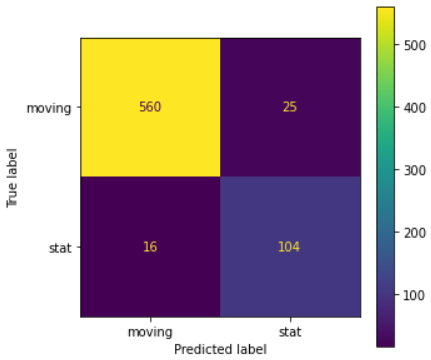
\includegraphics[scale = 0.7]{Images/cm knn3 mov stat.PNG}
\caption{Confusion matrix for the kNN (k = 3).}
\end{subfigure}
\hfill
\begin{subfigure}{.45\textwidth}
\centering
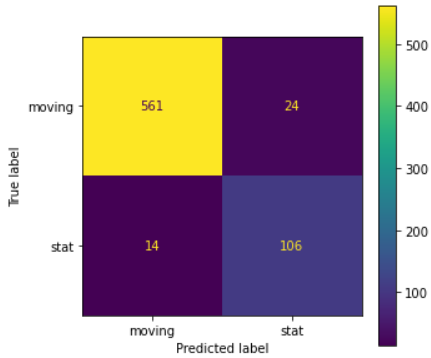
\includegraphics[scale = 0.7]{Images/cm knn5 mov stat.PNG}
\caption{Confusion matrix for the kNN (k = 5).}
\end{subfigure}
\medskip

\begin{subfigure}{.45\textwidth}
\centering
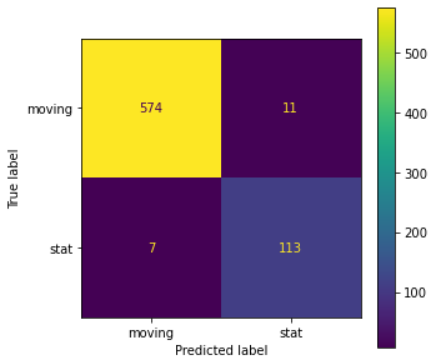
\includegraphics[scale = 0.7]{Images/cm svm mov stat.PNG}
\caption{Confusion matrix for the SVM.}
\end{subfigure}
\hfill
\begin{subfigure}{.45\textwidth}
\centering
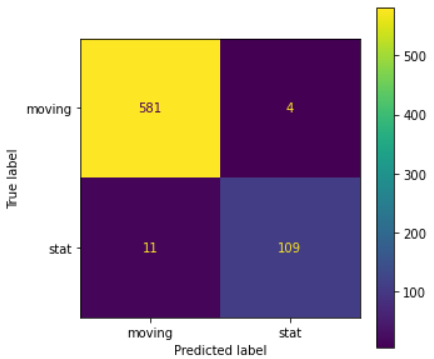
\includegraphics[scale = 0.7]{Images/cm xgb mov stat.PNG}
\caption{Confusion matrix for XGBoost.}
\end{subfigure}
\medskip

\begin{subfigure}{.45\textwidth}
\centering
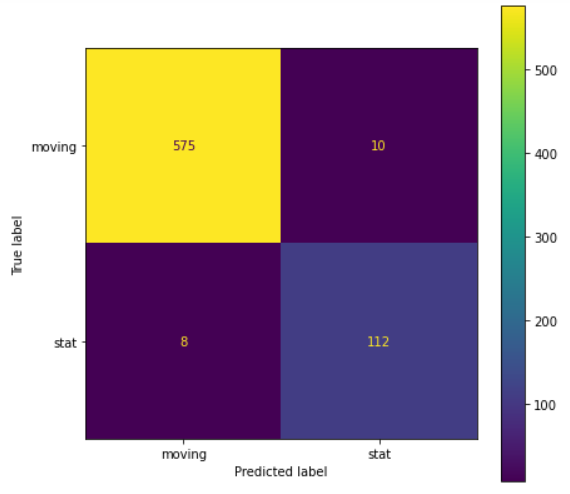
\includegraphics[scale = 0.52]{Images/cm nn mov stat.PNG}
\caption{Confusion matrix for the neural network.}
\end{subfigure}
\hfill
\begin{subfigure}{.5\textwidth}
\centering
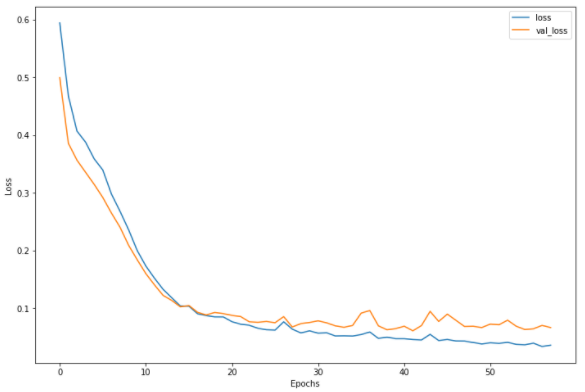
\includegraphics[scale = 0.55]{Images/loss nn mov stat.PNG}
\caption{Loss graph for the neural network.}
\end{subfigure}

\caption{Confusion matrices for the algorithms for task 1.}
\label{fig:cm_mov_stat}
\end{figure}
%

\clearpage
\section{The confusion matrices for Task 2}
\label{appendix:CM2}

%
\begin{figure}[ht]
\centering
\begin{subfigure}{.45\textwidth}
\centering
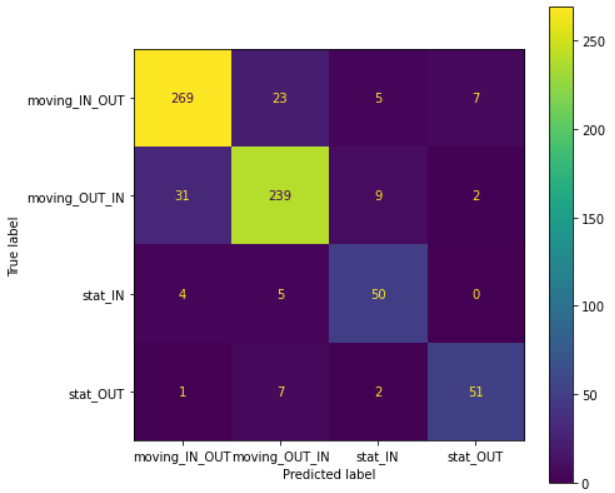
\includegraphics[scale = 0.55]{Images/cm knn3 in out.PNG}
\caption{Confusion matrix for the kNN (k = 3).}
\end{subfigure}
\hfill
\begin{subfigure}{.45\textwidth}
\centering
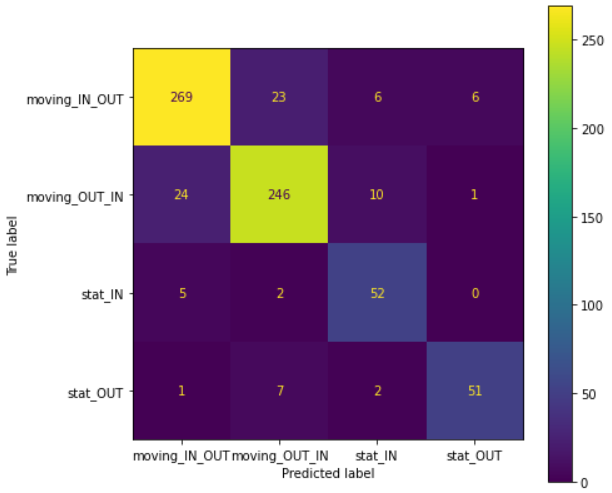
\includegraphics[scale = 0.55]{Images/cm knn5 in out.PNG}
\caption{Confusion matrix for the kNN (k = 5).}
\end{subfigure}
\medskip

\begin{subfigure}{.45\textwidth}
\centering
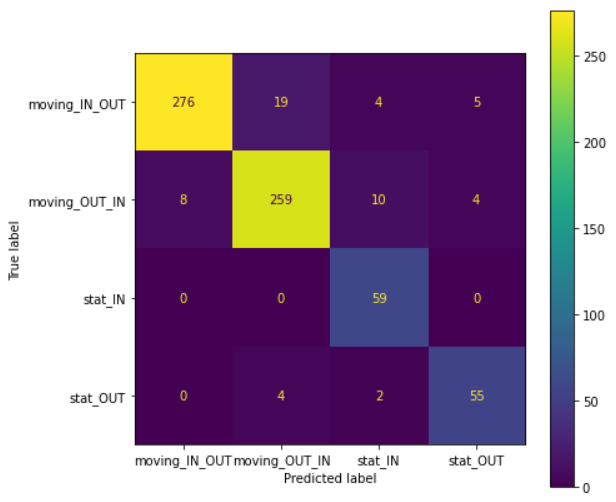
\includegraphics[scale = 0.55]{Images/cm svm in out.PNG}
\caption{Confusion matrix for the SVM.}
\end{subfigure}
\hfill
\begin{subfigure}{.45\textwidth}
\centering
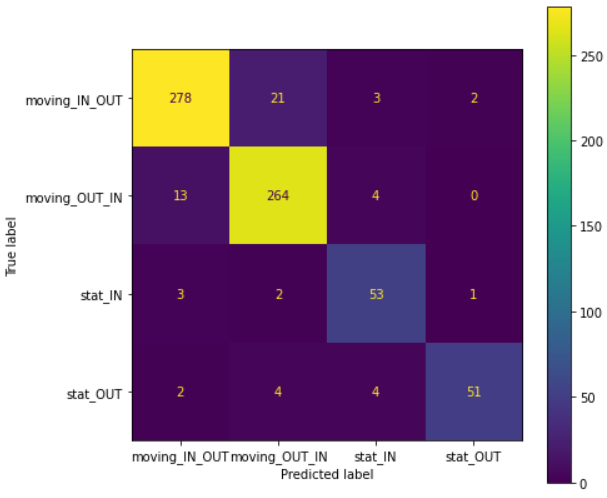
\includegraphics[scale = 0.55]{Images/cm xgb in out.PNG}
\caption{Confusion matrix for XGBoost.}
\end{subfigure}
\medskip

\begin{subfigure}{.45\textwidth}
\centering
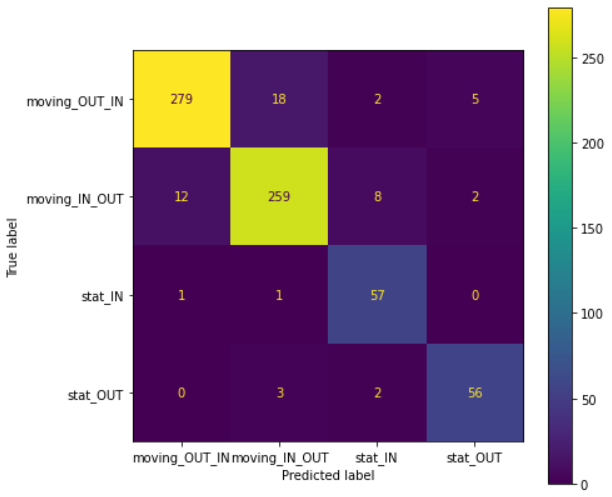
\includegraphics[scale = 0.55]{Images/cm nn in out.PNG}
\caption{Confusion matrix for the neural network.}
\end{subfigure}
\hfill
\begin{subfigure}{.45\textwidth}
\centering
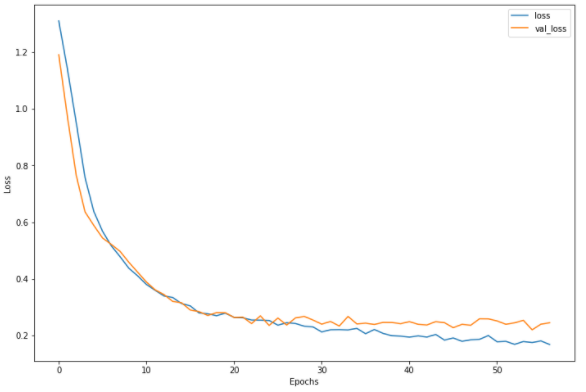
\includegraphics[scale = 0.55]{Images/loss nn in out.PNG}
\caption{Loss graph for the neural network.}
\end{subfigure}

\caption{Confusion matrices for the algorithms for task 2.}
\label{fig:cm_in_out}
\end{figure}
%

\clearpage
\section{The confusion matrices for Task 3}
\label{appendix:CM3}

%
\begin{figure}[ht]
\centering
\begin{subfigure}{.45\textwidth}
\centering
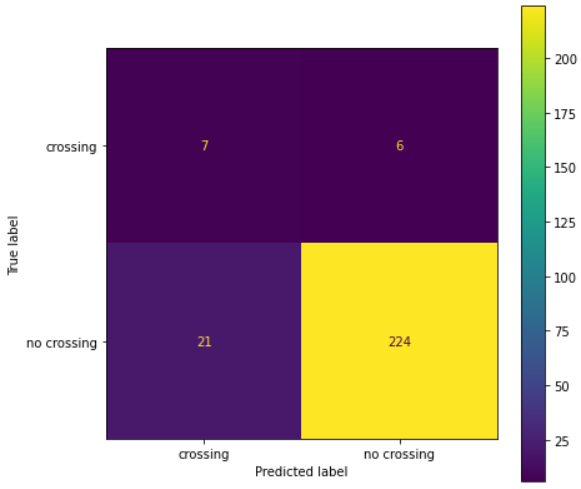
\includegraphics[scale = 0.55]{Images/cm knn3 crossing.PNG}
\caption{Confusion matrix for the kNN (k = 3).}
\end{subfigure}
\hfill
\begin{subfigure}{.45\textwidth}
\centering
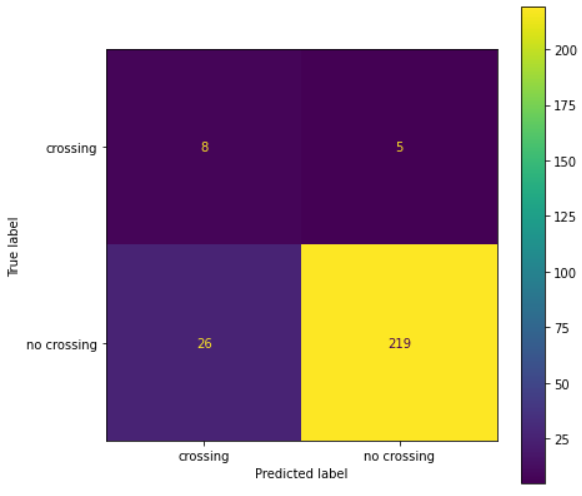
\includegraphics[scale = 0.55]{Images/cm knn5 crossing.PNG}
\caption{Confusion matrix for the kNN (k = 5).}
\end{subfigure}
\medskip

\begin{subfigure}{.45\textwidth}
\centering
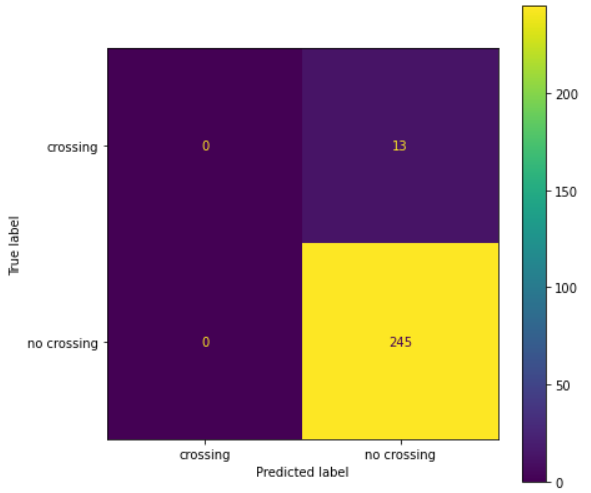
\includegraphics[scale = 0.55]{Images/cm svm crossing.PNG}
\caption{Confusion matrix for the SVM.}
\end{subfigure}
\hfill
\begin{subfigure}{.45\textwidth}
\centering
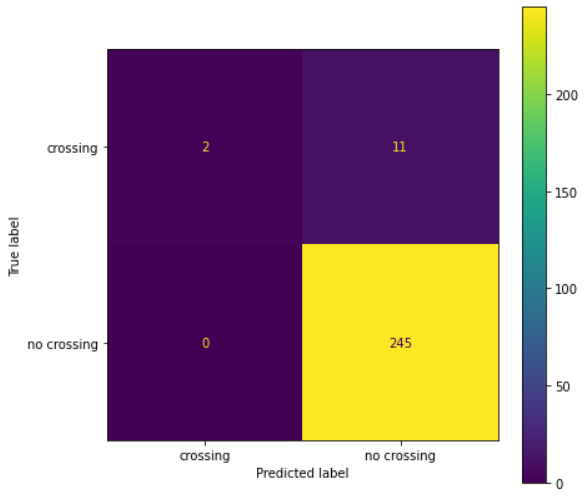
\includegraphics[scale = 0.55]{Images/cm xgb crossing.PNG}
\caption{Confusion matrix for XGBoost.}
\end{subfigure}
\medskip

\begin{subfigure}{.45\textwidth}
\centering
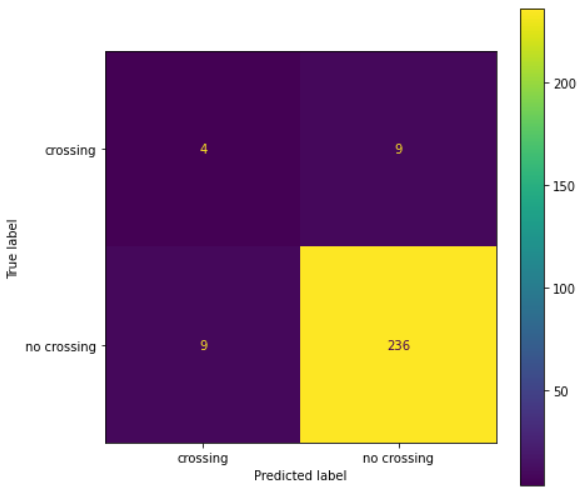
\includegraphics[scale = 0.55]{Images/cm nn crossing.PNG}
\caption{Confusion matrix for the neural network.}
\end{subfigure}
\hfill
\begin{subfigure}{.45\textwidth}
\centering
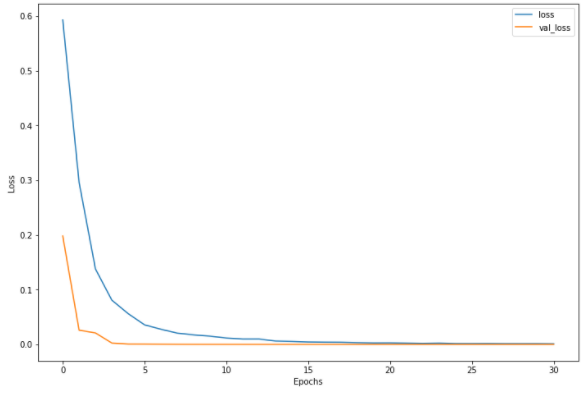
\includegraphics[scale = 0.55]{Images/loss nn crossing.PNG}
\caption{Loss graph for the neural network.}
\end{subfigure}

\caption{Confusion matrices for the algorithms for task 3.}
\label{fig:cm_crossing}
\end{figure}
%

\end{document}
